\section{Evaluation of main MPPT techniques\label{MPPTalgo}}

\subsection{Constant voltage algorithm}
Empirical experiments have shown that the voltage has a linear dependence on the MPP at different ambient conditions. The MPP is in the range of 70 to 80 of the open circuit voltage. The advantage of this algorithm is that only the voltage is measured and the control of the system is done by a simple control loop. The location of such PV-panels with the constant voltage as MPP algorithm is only possible in regions with low temperature fluctuations. The reason for this disadvantage is that with strong temperature fluctuations the point of the MPP varies very strongly and the assumption of linear dependence is no longer valid. In addition, it does not work with PV panels which are partially shaded.\cite{}

\subsection{Perturb and Observe}
Perturb and observe is with the incremental conductance the most frequently used algorithm for MPPT. With perturb and observe, the currently measured power is periodically compared with the previous power. If the measured power is greater than the power from the previous measurement, the voltage is further increased to reach the MPP. If a power reduction is detected after the comparison, the voltage is reduced. The flowchart in the figure \ref{fcperturbandobserve} illustrates this method. The classical algorithm uses a fixed step to change the voltage. When the MPP is reached, the algorithm oscillates around the MPP. If the fixed step value is high, the MPP is reached quickly. On the other hand, the oscillation around the MPP is high, which reduces the efficiency. The advantage of a small value is that the oscillation is smaller, but it takes more time to reach the MPP.

\begin{figure}[htbp]
	\begin{center}
		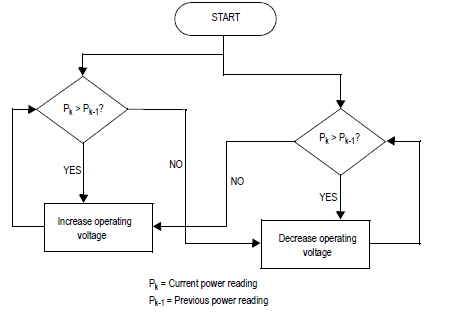
\includegraphics[width=0.7\textwidth]{../Pictures/flow_chart_perturb_observe}
		\caption{flow chart from perturb and observe.picture should change }
		\label{fcperturbandobserve}
	\end{center}	
\end{figure}

\subsection{Incremental conductancee}
The approach of incremental conductance is that the MPP is at the position where the derivative of power after voltage is 0. The left side of the MPP is the derivative greater than 0 and the right side is the derivative less than 0, which is what the equations describe. The algorithm compares the incremental conductance with the previous one to then increase (left side of the MPP) or decrease (left side of the MPP) the voltage.  In this procedure, the algorithm is stopped when the MPP is reached. There is no oscillation around the MPP. If a change in current is detected, the algorithm starts to find the MPP again, as you can see in the flowchart in figure \ref{fcincrementalc}. As with perturb and observe, a fixed value is used to change the voltage. If the value is high, the probability is higher that the algorithm oscillates around the MPP. 

